\documentclass[a4paper]{scrartcl}
\usepackage{mathe-blatt}
\usepackage{graphicx}
\usepackage{listings}
\blattnumeins

\begin{document}

\begin{aufgabe}~

	Seien die Koeffizienten des Polynoms $p\in \P_3$ gegeben durch
	\[
		p(x) = ax^3 + bx^2 + cx + d
	\]
	Es folgt
	\begin{align*}
		p'(x) &= 3ax^2 + 2bx + c \\
		p''(x) &= 6ax + 2b
	\end{align*}
	\begin{enumerate}[a)]
		\item
			Aus $p(0)=1$ und $p''(0)=1$ ergibt sich sofort $d=1, b=\f 12$.
			Außerdem für $p(1)=1$ und $p'(1)=1$ die Gleichungen
			\begin{align*}
				a + 1 + c + 1 &= 1\\
				3a + 2 + c &= 1
			\end{align*}
			Also $a=0$ und $c=-1$.
			Das gesuchte Polynom ist also eindeutig gegeben durch
			\[
				p(x) = \f 12 x^2 -x +1
			\]
		\item
			Aus $p(0)=0$ und $p'(0)=1$ ergibt sich sofort $d=0, c=1$.
			Für $\int_{-1}^1 p(x) dx = 1$ ergibt sich die Gleichung
			\[
				1 = \int_{-1}^1 ax^3 + bx^2 + x dx = \left[ \f a4 x^4 + \f b3 x^3 + \f 12 x^2\right]_{-1}^1
				= \f 23 b
			\]
			also $b=\f 32$.
			Der Parameter $a\in \R$ kann beliebig gewählt werden.
			Die gesuchten Polynome sind also alle in der Menge
			\[
				\left\{ax^3+\f 32 x^2 + x \in \P_3 : a\in \R \right\}
			\]
		\item
			Aus $p'(0)=0$ und $p''(0)=2$ folgt sofort $c=0, b=1$.
			Für $p'(1)=1$ und $p''(1)=6$ ergeben sich die Gleichungen
			\begin{align*}
				3a + 2 &= 1 \\
				6a + 2 &= 6
			\end{align*}
			bzw. $a=-\f 13$ und $a=\f 23$, ein Widerspruch.
			Es gibt also kein Polynom in $\P_3$, das die geforderten Bedingungen erfüllt.
	\end{enumerate}		
\end{aufgabe}

\begin{aufgabe}
		\begin{enumerate}[a)]
			\item
				Angenommen, es gäbe ein lineares Polynom $p(x,y) = ax + by + c$, welches die angegebenen Werte annimmt, dann müsste gelten:
				\begin{align*}
					0 = z_1 = p(1,0) &= a \\
					-1 = z_2 = p(0,1) &= b \\
					1 = z_3 = p(1,1) &= a + b = -1
				\end{align*}
				ein Widerspruch.
				Es kann also kein lineares Polynom existieren, dass die gewünschten Werte annimmt.
			\item
				Sei
				\[
					p(x,y) = ax^2 + bxy + cy^2 + dx + ey + f
				\]
				ein quadratisches Polynom.
				Damit dieses die erforderlichen Werte annimmt, muss gelten
				\begin{align*}
					0 = z_0 = p(0,0) &= f \\
					0 = z_1 = p(1,0) &= a + d \\
					-1 = z_2 = p(0,1) &= c + e \\
					1 = z_3 = p(1,1) &= a + b + c + d + e
				\end{align*}
				Da
				\begin{align*}
					p(x,0) = ax^2 + dx \\
					p(0,y) = cy^2 + ey
				\end{align*}
				quadratische Polynome sein sollen, folgt zwangsläufig $a=0$ und $c=0$.
				Aus den Punktgleichungen oben deshalb auch $d=0$ und $e=-1$, sowei $b=2$.
				Das gesuchte Polynom ist also gegeben durch
				\[
					p(x,y) = 2xy - y
				\]
			\item
				Da jedes Polynom eindeutig durch seine Koeffizienten in der Monombasis gegeben ist und diese eindeutig im Teil b) bestimmt wurden, ist das Polynom eindeutig gegeben.
		\end{enumerate}
\end{aufgabe}

\begin{aufgabe}
	\begin{enumerate}[a)]
		\item
			Es gilt
			\[
				\scr F_N(a\mathbf f + b\mathbf g) = \f 1N W_N (a\mathbf f + b\mathbf g) = a\f 1N W_N \mathbf f + b \f 1N W_N \mathbf g = a \scr F_N(\mathbf f) + b \scr F_N(\mathbf g) = a\mathbf c + b\mathbf d
			\]
		\item
	\end{enumerate}
\end{aufgabe}
\newpage
\begin{aufgabe}~

	\begin{enumerate}[a)]
		\item
			Die Routine lautet (Matlab):
			\begin{lstlisting}[language=matlab]
function [px, py] = my2dinterpol(x, y)
	n = length(x) - 1;
	px = polyfit(0:n, x, n);
	py = polyfit(0:n, y, n);
end
			\end{lstlisting}
		\item
			Code zum Testen der Routine (Matlab):
			\begin{lstlisting}[language=matlab]
n = 8;
[px, py] = my2dinterpol([1,3,5,6,8,7,4,2,1], [4,3,2,1,4,7,6,5,4]);
plot(...
	polyval(px, linspace(0,n)), polyval(py, linspace(0,n)), 'b-', ...
	polyval(px, 0:n), polyval(py, 0:n), 'r.' ...
);
			\end{lstlisting}
			\begin{figure*}[h]
				\centering
				\caption{2D Kurvenplot des Interpolationspolynoms ($t\in [0,n]$)}
				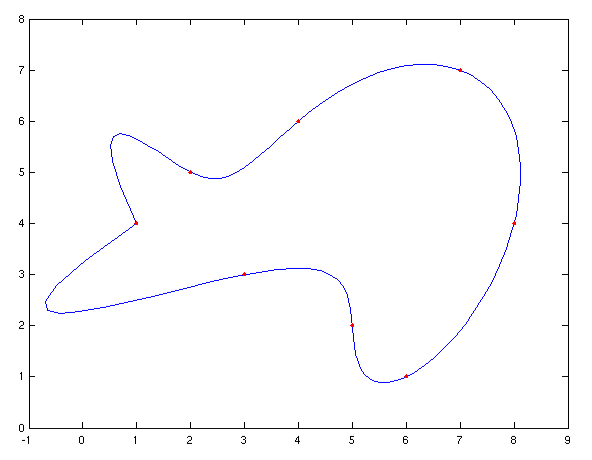
\includegraphics[scale=0.7]{num1_3_4}
			\end{figure*}
		\item
			Die Kurve $(p_x(t),p_y(t))$ für $t\in[0,n]$ ist eine geschwungene Linie, die durch alle angegebenen Punkte geht.
			Sie hat einzig beim Anfangs/Endpunkt $(1,4)$ einen Knick.
	\end{enumerate}

\end{aufgabe}

\end{document}
